	\chapter{Système de propulsion}

	Le principe fondamental de déplacement de l'aéroglisseur est basé sur la rotation d'une hélice, qui génèrera le flux d'air nécessaire au déplacement de l'aéroglisseur.
	
	La mise en rotation de cette hélice sera réalisée grâce à un moteur DC brushless. 
	
	Après avoir présenté quelques généralités sur le moteur DC  brushless
		
	Le \textbf{moteur DC brushless} (en anglais \textit{Brushless DC Motor}, abrégé BLDCM par la suite) est un moteur qui a connu un gain en popularité très important au cours des deux dernières décennies. Et pour cause, les champs d'application de ce type de moteur sont multiples : appareils électroménagers, automobile, aérospatial, équipement médical, production industrielle et instrumentation \cite{AN885}. 
			
	Le moteur \textbf{NM Prodrive 3350 110kV} retenu pour la conception de notre aéroglisseur est un moteur DC brushless. Il sera notamment utilisé dans notre système pour la rotation de l'hélice, qui permettra à la fois la propulsion et la génération du flux d'air nécessaire à la création du coussin d'air qui supportera l'aéroglisseur.
			
	Dans cette partie, nous développerons dans un premier temps les généralités autour des moteurs DC brushless. Dans un second et troisième temps, nous aborderons les aspects de conception d'un onduleur et de contrôle du moteur avec une méthode ne faisant appel à aucun capteur basée sur la lecture du retour de force électromécanique. Une quatrième partie se concentrera sur les aspects de réalisation d'un PCB de contrôle 
			
		\section{Généralités sur le moteur à courant continu \textit{brushless}}
			
		Comme son nom l'indique, et contrairement à la majorité des moteurs à courant continu, le \textbf{moteur à courant continu \textit{brushless}} (en anglais \textit{Brushless DC Motor}, abrégé BLDCM par la suite) \textbf{n'utilise pas de balais}. Les moteurs à courant continu standards disposent en effet de bobinages sur le rotor et nécessitent donc un \textbf{collecteur} constitué de balais pour alimenter ces bobinages. Cependant, ce collecteur est source de nombreux désagréments. Cette pièce est soumise à l'usure et réduit considérablement la longévité des moteurs à courant continu. De plus, cette pièce assurant la transmission d'énergie électrique vers le rotor est sujette à des pertes énergétiques, qu'elles soient mécaniques ou électriques. 
		
		Historiquement, le moteur à courant continu a toujours été populaire du fait de la facilité de réglage de la vitesse ou du couple de sortie. Les moteurs asynchrones, quant-à-eux Les innovations dans les champs de l'électronique de puissance, mais aussi l'apparition progressive des microprocesseurs aves des capacités de calcul de plus en plus importantes permettent par la suite une ouverture à de nouvelles possibilités de contrôle des moteurs. 
		
		
		
		
	
	
	 La commutation est au contraire réalisée électroniquement. L'utilisation de cette structure fait que le BLDCM a de nombreux avantages par rapport aux moteurs DC à balais ou les moteurs à induction. Parmi ces avantages, on peut notamment retenir :
			
			
		Les avantages de l'utilisation des moteurs \textit{brushless} sont nombreux. L'absence de balais permet 
	
			
			De plus, le rapport couple délivré / encombrement moteur est amélioré, ce qui rend le BLDCM très utile dans des applications où l'espace et le poids sont des critères cruciaux \cite{AN885}, comme dans le cas de notre aéroglisseur.
			
	
			
			\subsection{Structure du moteur brushless}
			
				
				 Un moteur brushless est structuré à partir d'un aimant permanent au rotor et de pôles bobinés au stator. L'énergie électrique est convertie en énergie mécanique par le biais des forces d'attraction magnétique entre l'aimant permanent du rotor et le champ tournant induit par les pôles bobinés du stator. La \textsc{Figure \ref{struct_bldcm}} présente une illustration simplifiée de la construction d'un BLDCM. 
				 
				 \begin{figure}
				 	\begin{center}
				 		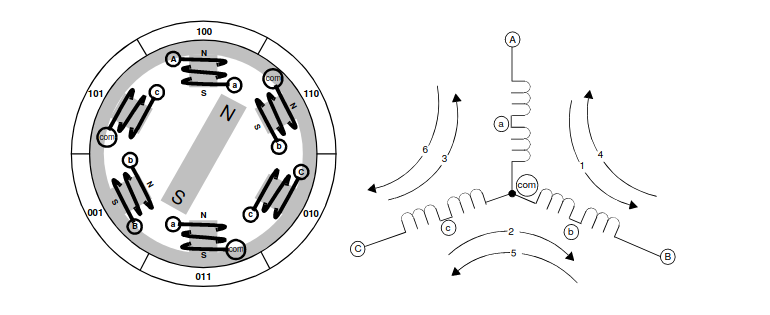
\includegraphics[scale=0.7]{../Illus/struct_bldcm.png}
				 	\end{center}
				 	\caption{Diagramme simplifié de la structure d'un BLDCM (\textit{Source :} \cite{AN857})}
				 	\label{struct_bldcm}
				 \end{figure}
				 
				 L'exemple de structure présenté ici montre trois circuits électromagnétiques connectés à un point commun (couplage étoile). Chacun des circuits est divisé en deux parties qui seront bobinées sur des dents de la machine diamétralement opposées. Cette structure permet alors à l'aimant permanent au rotor de se déplacer au milieu de champs magnétiques induits. Nous avons modélisé le BLDCM en utilisant le logiciel \textit{FEMM} pour donner une idée plus concrète de son fonctionnement en rotation. La montre notamment la modélisation de la structure du moteur sur ce logiciel.
				 
				 \subsection{Modélisation}
				 
				 % Capture d'écran structure FEMM électif circuit magnétique

				 La plupart des BLDCM ont une structure triphasée avec un couplage étoile, et c'est notamment le cas du moteur que nous allons utiliser dans ce projet. Un tel moteur est alors piloté en alimentant deux phases en même temps. Afin d'entrer en rotation, les trois phases du moteur devront être alimentées 
				 
				 \subsection{Séquence de commutation}
				 
				  % Récupérer modélisation FEMM de l'électif circuits magnétiques S4
				  
				 \subsubsection{Structure d'un onduleur triphasé}
				 
				 \subsection{•}
				 
				 \subsection{•}
				 
		\section{Modélisation électrique du système de propulsion}
			
		Le système complet de propulsion va être modélisé sous le logiciel \textit{PSIM}.
			
			\subsection{Modélisation de l'onduleur triphasé} 
				
			\subsection{Modélisation du moteur DC brushless}
				
					\paragraph{Angle d'avance}
					C'est un paramètre de simulation très important si l'on veut pouvoir accéder à des vitesses de rotation intéressantes pour notre système. Afin de mieux présenter ce paramètre et de comprendre son sens physique, nous allons proposer ici une analogie avec l'avance à l'allumage d'un moteur thermique.
					
					Avec une avance nulle l'etincelle arrive juste quand le piston est en haut du cylindre. Le front de flamme aidera juste à pousser le piston dans sa redescente: ca marche mais c'est pas optimisé. SI on met de l'avance l'éticelle commencera à emflammer le mélange un peu avant que le piston soit au point mort haut alors le front de flamme déja bien avancé quand le piston arrivera et il aura ainsi plus de patate pour redescendre car la pression sera plus forte.
En mettant encore plus d'avance, donc en avancant encore plus le moment où l'etincelle approche le piston va forcer un peu pour finir de monter (entrainé par les autres pistons ou par son inertie) pour finalement "rebondir" sur le melange deja en grande partie dilaté. Il ne faut pas aller plus loin car il risque d'y avoir des retours ou des claquements.


Tu remarqueras que ce temps d'avance (timing) depend de la vitesse de rotation, plus le moteur tourne vite plus il faut declencher tot, et c'est là que les allumages electroniques "intelligents" ont pris le pas sur les simples vis platinées. (c'est notemment grace à ces reglages qu'on peut optimiser sa BMW par exemple avec l'ajout de la fameuse "puce" qui definit des diagrammes de timings).

En electrique c'est pareil, soft timing: tu suis juste le mouvement, medium timing tu optimises pour "aller chercher" le rotor, et hard timing tu "forces" presque l'etat suivant avant que celui ci soit fini.
Ici l' "etincelle" c'est l'alimentation des bobines et le piston c'est un pole du rotor.

on notera que hard timing: surtout pour les cages tournantes.

					L'angle d'avance est un paramètre à régler en prenant également en compte le nombre de paires de pôles du moteur utilisé.
		
			
			
				\subsection{Modélisation de l'hélice}
				
				L'hélice est également prise en compte dans la simulation 
				
				
				 
		\subsection{Conception de l'onduleur triphasé}
		
		\subsection{Résultats de simulation}
		
		
	\section{Réalisation des PCBs}
		
			\subsubsection{Calcul des surfaces d'échange}			
			
			\subsubsection{Capacité de découplage}
				 
				 \subsection{Méthode de contrôle du BLDCM}
				 
				 Le BLDCM que nous avons retenu pour 
				 
				 	\subsubsection{t}
				 
				 
				 
				 
				 
				 
				 
				 
				 

			
			\subsection{Contrôle basé sur le retour de force électromotrice}
			\newcommand{\pic}{\texttt{PIC16F1619} }
			\newcommand{\dspic}{\texttt{dsPIC30F2010} }